% Created by tikzDevice version 0.12.3.1 on 2023-05-29 23:50:24
% !TEX encoding = UTF-8 Unicode
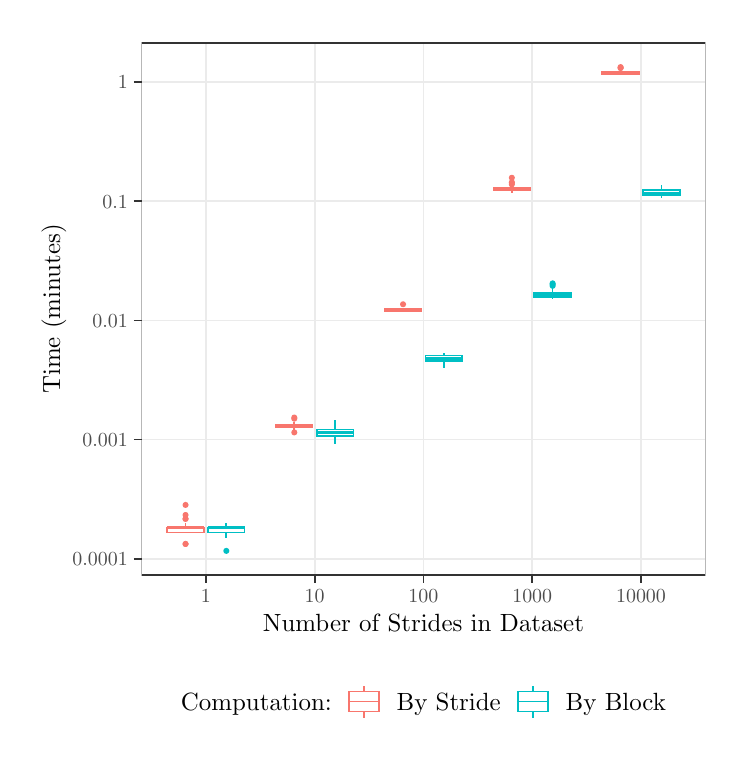
\begin{tikzpicture}[x=1pt,y=1pt]
\definecolor{fillColor}{RGB}{255,255,255}
\path[use as bounding box,fill=fillColor,fill opacity=0.00] (0,0) rectangle (250.38,261.76);
\begin{scope}
\path[clip] (  0.00,  0.00) rectangle (250.38,261.76);
\definecolor{drawColor}{RGB}{255,255,255}
\definecolor{fillColor}{RGB}{255,255,255}

\path[draw=drawColor,line width= 0.6pt,line join=round,line cap=round,fill=fillColor] ( -0.00, -0.00) rectangle (250.38,261.76);
\end{scope}
\begin{scope}
\path[clip] ( 41.14, 63.96) rectangle (244.88,256.26);
\definecolor{fillColor}{RGB}{255,255,255}

\path[fill=fillColor] ( 41.14, 63.96) rectangle (244.88,256.26);
\definecolor{drawColor}{gray}{0.92}

\path[draw=drawColor,line width= 0.6pt,line join=round] ( 41.14, 69.82) --
	(244.88, 69.82);

\path[draw=drawColor,line width= 0.6pt,line join=round] ( 41.14,112.89) --
	(244.88,112.89);

\path[draw=drawColor,line width= 0.6pt,line join=round] ( 41.14,155.96) --
	(244.88,155.96);

\path[draw=drawColor,line width= 0.6pt,line join=round] ( 41.14,199.03) --
	(244.88,199.03);

\path[draw=drawColor,line width= 0.6pt,line join=round] ( 41.14,242.11) --
	(244.88,242.11);

\path[draw=drawColor,line width= 0.6pt,line join=round] ( 64.41, 63.96) --
	( 64.41,256.26);

\path[draw=drawColor,line width= 0.6pt,line join=round] (103.71, 63.96) --
	(103.71,256.26);

\path[draw=drawColor,line width= 0.6pt,line join=round] (143.01, 63.96) --
	(143.01,256.26);

\path[draw=drawColor,line width= 0.6pt,line join=round] (182.32, 63.96) --
	(182.32,256.26);

\path[draw=drawColor,line width= 0.6pt,line join=round] (221.62, 63.96) --
	(221.62,256.26);
\definecolor{drawColor}{RGB}{248,118,109}
\definecolor{fillColor}{RGB}{248,118,109}

\path[draw=drawColor,line width= 0.4pt,line join=round,line cap=round,fill=fillColor] ( 57.04, 89.30) circle (  0.89);

\path[draw=drawColor,line width= 0.4pt,line join=round,line cap=round,fill=fillColor] ( 57.04, 84.28) circle (  0.89);

\path[draw=drawColor,line width= 0.4pt,line join=round,line cap=round,fill=fillColor] ( 57.04, 84.28) circle (  0.89);

\path[draw=drawColor,line width= 0.4pt,line join=round,line cap=round,fill=fillColor] ( 57.04, 85.67) circle (  0.89);

\path[draw=drawColor,line width= 0.4pt,line join=round,line cap=round,fill=fillColor] ( 57.04, 75.20) circle (  0.89);

\path[draw=drawColor,line width= 0.4pt,line join=round,line cap=round,fill=fillColor] ( 57.04, 75.20) circle (  0.89);

\path[draw=drawColor,line width= 0.6pt,line join=round] ( 57.04, 81.16) -- ( 57.04, 82.78);

\path[draw=drawColor,line width= 0.6pt,line join=round] ( 57.04, 79.37) -- ( 57.04, 79.37);
\definecolor{fillColor}{RGB}{255,255,255}

\path[draw=drawColor,line width= 0.6pt,fill=fillColor] ( 50.40, 81.16) --
	( 50.40, 79.37) --
	( 63.67, 79.37) --
	( 63.67, 81.16) --
	( 50.40, 81.16) --
	cycle;

\path[draw=drawColor,line width= 1.1pt] ( 50.40, 81.16) -- ( 63.67, 81.16);
\definecolor{fillColor}{RGB}{248,118,109}

\path[draw=drawColor,line width= 0.4pt,line join=round,line cap=round,fill=fillColor] ( 96.34,120.89) circle (  0.89);

\path[draw=drawColor,line width= 0.4pt,line join=round,line cap=round,fill=fillColor] ( 96.34,120.47) circle (  0.89);

\path[draw=drawColor,line width= 0.4pt,line join=round,line cap=round,fill=fillColor] ( 96.34,115.50) circle (  0.89);

\path[draw=drawColor,line width= 0.6pt,line join=round] ( 96.34,118.27) -- ( 96.34,119.41);

\path[draw=drawColor,line width= 0.6pt,line join=round] ( 96.34,117.31) -- ( 96.34,116.04);
\definecolor{fillColor}{RGB}{255,255,255}

\path[draw=drawColor,line width= 0.6pt,fill=fillColor] ( 89.71,118.27) --
	( 89.71,117.31) --
	(102.97,117.31) --
	(102.97,118.27) --
	( 89.71,118.27) --
	cycle;

\path[draw=drawColor,line width= 1.1pt] ( 89.71,117.56) -- (102.97,117.56);
\definecolor{fillColor}{RGB}{248,118,109}

\path[draw=drawColor,line width= 0.4pt,line join=round,line cap=round,fill=fillColor] (135.64,161.81) circle (  0.89);

\path[draw=drawColor,line width= 0.6pt,line join=round] (135.64,160.10) -- (135.64,160.51);

\path[draw=drawColor,line width= 0.6pt,line join=round] (135.64,159.35) -- (135.64,158.93);
\definecolor{fillColor}{RGB}{255,255,255}

\path[draw=drawColor,line width= 0.6pt,fill=fillColor] (129.01,160.10) --
	(129.01,159.35) --
	(142.28,159.35) --
	(142.28,160.10) --
	(129.01,160.10) --
	cycle;

\path[draw=drawColor,line width= 1.1pt] (129.01,159.76) -- (142.28,159.76);
\definecolor{fillColor}{RGB}{248,118,109}

\path[draw=drawColor,line width= 0.4pt,line join=round,line cap=round,fill=fillColor] (174.95,205.89) circle (  0.89);

\path[draw=drawColor,line width= 0.4pt,line join=round,line cap=round,fill=fillColor] (174.95,205.70) circle (  0.89);

\path[draw=drawColor,line width= 0.4pt,line join=round,line cap=round,fill=fillColor] (174.95,207.53) circle (  0.89);

\path[draw=drawColor,line width= 0.4pt,line join=round,line cap=round,fill=fillColor] (174.95,205.13) circle (  0.89);

\path[draw=drawColor,line width= 0.6pt,line join=round] (174.95,203.79) -- (174.95,205.07);

\path[draw=drawColor,line width= 0.6pt,line join=round] (174.95,202.91) -- (174.95,202.19);
\definecolor{fillColor}{RGB}{255,255,255}

\path[draw=drawColor,line width= 0.6pt,fill=fillColor] (168.32,203.79) --
	(168.32,202.91) --
	(181.58,202.91) --
	(181.58,203.79) --
	(168.32,203.79) --
	cycle;

\path[draw=drawColor,line width= 1.1pt] (168.32,203.35) -- (181.58,203.35);
\definecolor{fillColor}{RGB}{248,118,109}

\path[draw=drawColor,line width= 0.4pt,line join=round,line cap=round,fill=fillColor] (214.25,247.22) circle (  0.89);

\path[draw=drawColor,line width= 0.4pt,line join=round,line cap=round,fill=fillColor] (214.25,247.52) circle (  0.89);

\path[draw=drawColor,line width= 0.4pt,line join=round,line cap=round,fill=fillColor] (214.25,247.20) circle (  0.89);

\path[draw=drawColor,line width= 0.6pt,line join=round] (214.25,245.94) -- (214.25,246.85);

\path[draw=drawColor,line width= 0.6pt,line join=round] (214.25,245.12) -- (214.25,244.99);
\definecolor{fillColor}{RGB}{255,255,255}

\path[draw=drawColor,line width= 0.6pt,fill=fillColor] (207.62,245.94) --
	(207.62,245.12) --
	(220.88,245.12) --
	(220.88,245.94) --
	(207.62,245.94) --
	cycle;

\path[draw=drawColor,line width= 1.1pt] (207.62,245.56) -- (220.88,245.56);
\definecolor{drawColor}{RGB}{0,191,196}
\definecolor{fillColor}{RGB}{0,191,196}

\path[draw=drawColor,line width= 0.4pt,line join=round,line cap=round,fill=fillColor] ( 71.78, 72.70) circle (  0.89);

\path[draw=drawColor,line width= 0.6pt,line join=round] ( 71.78, 81.16) -- ( 71.78, 82.78);

\path[draw=drawColor,line width= 0.6pt,line join=round] ( 71.78, 79.37) -- ( 71.78, 77.40);
\definecolor{fillColor}{RGB}{255,255,255}

\path[draw=drawColor,line width= 0.6pt,fill=fillColor] ( 65.14, 81.16) --
	( 65.14, 79.37) --
	( 78.41, 79.37) --
	( 78.41, 81.16) --
	( 65.14, 81.16) --
	cycle;

\path[draw=drawColor,line width= 1.1pt] ( 65.14, 81.16) -- ( 78.41, 81.16);

\path[draw=drawColor,line width= 0.6pt,line join=round] (111.08,116.56) -- (111.08,119.84);

\path[draw=drawColor,line width= 0.6pt,line join=round] (111.08,114.17) -- (111.08,111.26);

\path[draw=drawColor,line width= 0.6pt,fill=fillColor] (104.45,116.56) --
	(104.45,114.17) --
	(117.71,114.17) --
	(117.71,116.56) --
	(104.45,116.56) --
	cycle;

\path[draw=drawColor,line width= 1.1pt] (104.45,115.50) -- (117.71,115.50);

\path[draw=drawColor,line width= 0.6pt,line join=round] (150.38,143.24) -- (150.38,144.20);

\path[draw=drawColor,line width= 0.6pt,line join=round] (150.38,141.42) -- (150.38,138.90);

\path[draw=drawColor,line width= 0.6pt,fill=fillColor] (143.75,143.24) --
	(143.75,141.42) --
	(157.02,141.42) --
	(157.02,143.24) --
	(143.75,143.24) --
	cycle;

\path[draw=drawColor,line width= 1.1pt] (143.75,142.36) -- (157.02,142.36);
\definecolor{fillColor}{RGB}{0,191,196}

\path[draw=drawColor,line width= 0.4pt,line join=round,line cap=round,fill=fillColor] (189.69,169.37) circle (  0.89);

\path[draw=drawColor,line width= 0.4pt,line join=round,line cap=round,fill=fillColor] (189.69,168.99) circle (  0.89);

\path[draw=drawColor,line width= 0.4pt,line join=round,line cap=round,fill=fillColor] (189.69,168.47) circle (  0.89);

\path[draw=drawColor,line width= 0.6pt,line join=round] (189.69,165.95) -- (189.69,168.21);

\path[draw=drawColor,line width= 0.6pt,line join=round] (189.69,164.38) -- (189.69,163.65);
\definecolor{fillColor}{RGB}{255,255,255}

\path[draw=drawColor,line width= 0.6pt,fill=fillColor] (183.05,165.95) --
	(183.05,164.38) --
	(196.32,164.38) --
	(196.32,165.95) --
	(183.05,165.95) --
	cycle;

\path[draw=drawColor,line width= 1.1pt] (183.05,165.06) -- (196.32,165.06);

\path[draw=drawColor,line width= 0.6pt,line join=round] (228.99,203.13) -- (228.99,204.79);

\path[draw=drawColor,line width= 0.6pt,line join=round] (228.99,201.16) -- (228.99,200.31);

\path[draw=drawColor,line width= 0.6pt,fill=fillColor] (222.36,203.13) --
	(222.36,201.16) --
	(235.62,201.16) --
	(235.62,203.13) --
	(222.36,203.13) --
	cycle;

\path[draw=drawColor,line width= 1.1pt] (222.36,201.96) -- (235.62,201.96);
\definecolor{drawColor}{gray}{0.20}

\path[draw=drawColor,line width= 0.6pt,line join=round,line cap=round] ( 41.14, 63.96) rectangle (244.88,256.26);
\end{scope}
\begin{scope}
\path[clip] (  0.00,  0.00) rectangle (250.38,261.76);
\definecolor{drawColor}{gray}{0.30}

\node[text=drawColor,anchor=base east,inner sep=0pt, outer sep=0pt, scale=  0.72] at ( 36.19, 67.34) {0.0001};

\node[text=drawColor,anchor=base east,inner sep=0pt, outer sep=0pt, scale=  0.72] at ( 36.19,110.41) {0.001};

\node[text=drawColor,anchor=base east,inner sep=0pt, outer sep=0pt, scale=  0.72] at ( 36.19,153.48) {0.01};

\node[text=drawColor,anchor=base east,inner sep=0pt, outer sep=0pt, scale=  0.72] at ( 36.19,196.55) {0.1};

\node[text=drawColor,anchor=base east,inner sep=0pt, outer sep=0pt, scale=  0.72] at ( 36.19,239.63) {1};
\end{scope}
\begin{scope}
\path[clip] (  0.00,  0.00) rectangle (250.38,261.76);
\definecolor{drawColor}{gray}{0.20}

\path[draw=drawColor,line width= 0.6pt,line join=round] ( 38.39, 69.82) --
	( 41.14, 69.82);

\path[draw=drawColor,line width= 0.6pt,line join=round] ( 38.39,112.89) --
	( 41.14,112.89);

\path[draw=drawColor,line width= 0.6pt,line join=round] ( 38.39,155.96) --
	( 41.14,155.96);

\path[draw=drawColor,line width= 0.6pt,line join=round] ( 38.39,199.03) --
	( 41.14,199.03);

\path[draw=drawColor,line width= 0.6pt,line join=round] ( 38.39,242.11) --
	( 41.14,242.11);
\end{scope}
\begin{scope}
\path[clip] (  0.00,  0.00) rectangle (250.38,261.76);
\definecolor{drawColor}{gray}{0.20}

\path[draw=drawColor,line width= 0.6pt,line join=round] ( 64.41, 61.21) --
	( 64.41, 63.96);

\path[draw=drawColor,line width= 0.6pt,line join=round] (103.71, 61.21) --
	(103.71, 63.96);

\path[draw=drawColor,line width= 0.6pt,line join=round] (143.01, 61.21) --
	(143.01, 63.96);

\path[draw=drawColor,line width= 0.6pt,line join=round] (182.32, 61.21) --
	(182.32, 63.96);

\path[draw=drawColor,line width= 0.6pt,line join=round] (221.62, 61.21) --
	(221.62, 63.96);
\end{scope}
\begin{scope}
\path[clip] (  0.00,  0.00) rectangle (250.38,261.76);
\definecolor{drawColor}{gray}{0.30}

\node[text=drawColor,anchor=base,inner sep=0pt, outer sep=0pt, scale=  0.72] at ( 64.41, 54.05) {1};

\node[text=drawColor,anchor=base,inner sep=0pt, outer sep=0pt, scale=  0.72] at (103.71, 54.05) {10};

\node[text=drawColor,anchor=base,inner sep=0pt, outer sep=0pt, scale=  0.72] at (143.01, 54.05) {100};

\node[text=drawColor,anchor=base,inner sep=0pt, outer sep=0pt, scale=  0.72] at (182.32, 54.05) {1000};

\node[text=drawColor,anchor=base,inner sep=0pt, outer sep=0pt, scale=  0.72] at (221.62, 54.05) {10000};
\end{scope}
\begin{scope}
\path[clip] (  0.00,  0.00) rectangle (250.38,261.76);
\definecolor{drawColor}{RGB}{0,0,0}

\node[text=drawColor,anchor=base,inner sep=0pt, outer sep=0pt, scale=  0.90] at (143.01, 43.70) {Number of Strides in Dataset};
\end{scope}
\begin{scope}
\path[clip] (  0.00,  0.00) rectangle (250.38,261.76);
\definecolor{drawColor}{RGB}{0,0,0}

\node[text=drawColor,rotate= 90.00,anchor=base,inner sep=0pt, outer sep=0pt, scale=  0.90] at ( 11.70,160.11) {Time (minutes)};
\end{scope}
\begin{scope}
\path[clip] (  0.00,  0.00) rectangle (250.38,261.76);
\definecolor{fillColor}{RGB}{255,255,255}

\path[fill=fillColor] ( 49.88,  5.50) rectangle (236.15, 30.95);
\end{scope}
\begin{scope}
\path[clip] (  0.00,  0.00) rectangle (250.38,261.76);
\definecolor{drawColor}{RGB}{0,0,0}

\node[text=drawColor,anchor=base west,inner sep=0pt, outer sep=0pt, scale=  0.90] at ( 55.38, 15.13) {Computation:};
\end{scope}
\begin{scope}
\path[clip] (  0.00,  0.00) rectangle (250.38,261.76);
\definecolor{fillColor}{RGB}{255,255,255}

\path[fill=fillColor] (114.36, 11.00) rectangle (128.82, 25.45);
\end{scope}
\begin{scope}
\path[clip] (  0.00,  0.00) rectangle (250.38,261.76);
\definecolor{drawColor}{RGB}{248,118,109}

\path[draw=drawColor,line width= 0.6pt] (121.59, 12.45) --
	(121.59, 14.61);

\path[draw=drawColor,line width= 0.6pt] (121.59, 21.84) --
	(121.59, 24.01);
\definecolor{fillColor}{RGB}{255,255,255}

\path[draw=drawColor,line width= 0.6pt,fill=fillColor] (116.17, 14.61) rectangle (127.01, 21.84);

\path[draw=drawColor,line width= 0.6pt] (116.17, 18.23) --
	(127.01, 18.23);
\end{scope}
\begin{scope}
\path[clip] (  0.00,  0.00) rectangle (250.38,261.76);
\definecolor{fillColor}{RGB}{255,255,255}

\path[fill=fillColor] (175.46, 11.00) rectangle (189.91, 25.45);
\end{scope}
\begin{scope}
\path[clip] (  0.00,  0.00) rectangle (250.38,261.76);
\definecolor{drawColor}{RGB}{0,191,196}

\path[draw=drawColor,line width= 0.6pt] (182.68, 12.45) --
	(182.68, 14.61);

\path[draw=drawColor,line width= 0.6pt] (182.68, 21.84) --
	(182.68, 24.01);
\definecolor{fillColor}{RGB}{255,255,255}

\path[draw=drawColor,line width= 0.6pt,fill=fillColor] (177.26, 14.61) rectangle (188.10, 21.84);

\path[draw=drawColor,line width= 0.6pt] (177.26, 18.23) --
	(188.10, 18.23);
\end{scope}
\begin{scope}
\path[clip] (  0.00,  0.00) rectangle (250.38,261.76);
\definecolor{drawColor}{RGB}{0,0,0}

\node[text=drawColor,anchor=base,inner sep=0pt, outer sep=0pt, scale=  0.90] at (152.14, 15.13) {By Stride};
\end{scope}
\begin{scope}
\path[clip] (  0.00,  0.00) rectangle (250.38,261.76);
\definecolor{drawColor}{RGB}{0,0,0}

\node[text=drawColor,anchor=base,inner sep=0pt, outer sep=0pt, scale=  0.90] at (212.53, 15.13) {By Block};
\end{scope}
\end{tikzpicture}
